\newpage
\section{Proposal for Classification of Optimization Approaches}
\label{ch:Proposal}

\begin{figure}[t]
    \centering
    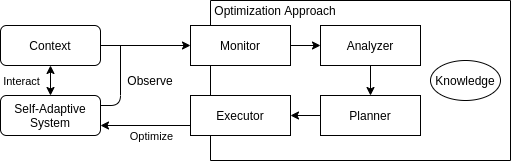
\includegraphics[width=0.8\textwidth]{images/ClassificationProposal-OptimizationMAPEK_horizontal.png}
    \caption{Mapping the optimization process to the \acrshort{mapek} feedback loop.}
    \label{fig:MappingOptMAPEK}
\end{figure}

This chapter will derive and propose a classification for \acrshort{oa} for \acrshort{sas}
based on concepts that were discussed in chapter \ref{ch:SASClassification}.
The main concepts that will be used for the classification of \acrshort{oa} are:
\begin{itemize}[nosep]
    \item The concept of using reflectiveness to describe \acrshort{sas}
    \item The 5W+1H questions to determine how a \acrshort{sas} operates
    \item The \acrshort{mapek} feedback loop as a general base for understanding \acrshort{sas}
    \item The concept of self-* properties which enables us to differentiate between self-adaptation
    and other self-* abilities
    \item A taxonomy for \acrshort{sas} which will be the basis for the proposed classification of \acrshort{oa},
    because \acrshort{sas} are so closely related to their \acrshort{oa}
\end{itemize}

\noindent Figure \ref{fig:MappingOptMAPEK} shows how an \acrshort{oa} for \acrshort{sas} can be understood as an additional reflective layer above the \acrshort{sas}.
Just like a \acrshort{sas}, the \acrshort{oa} has to monitor its environment or context and its subject.
In contrast to a \acrshort{sas} the \acrshort{oa} observes a \acrshort{sas} whose top level is a reflective layer and not a system whose top level is a base-level layer.
Similarly to the \acrshort{sas} the \acrshort{oa} has to analyze the data gathered by the \textit{Monitor} which is done by the \textit{Analyzer}.
After this the \textit{Planner} can plan an optimization which is then performed by the \textit{Executor}.
This optimization process happens with \textit{Knowledge} of the \acrshort{sas} and its environment.

\noindent This means that with the concept of layers of reflectiveness from FORMS \cite*{FORMS} and the \acrshort{mapek} feedback loop \cite*{VisionOfAutonomicComputing},
an \acrshort{oa} for a \acrshort{sas} can be understood as an \acrshort{sas} of a \acrshort{sas}.
Following this logic, a classification for \acrshort{oa} should be able to answer the same questions as a classification for \acrshort{sas}.
The main classification for \acrshort{sas} that this paper will focus on is the taxonomy for \acrshort{sas} by Krupitzer et al. \cite*{SurveyOnEngineeringApproaches}.
Because of this there are six questions that the classification for \acrshort{oa} has to be able to answer.
These are the 5W+1H questions by Salehie and Tahvildari \cite*{LandscapeAndResearchChallenges}: Where, When, What, Why, Who and How.

\begin{figure}[h]
    \centering
    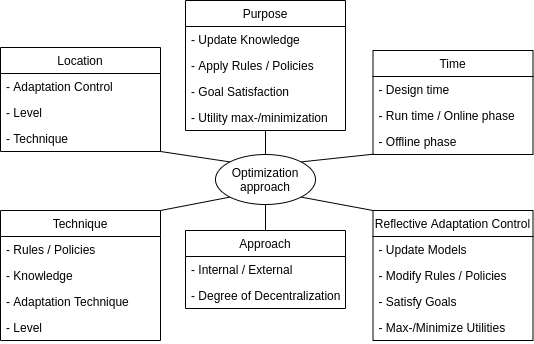
\includegraphics[width=0.8\textwidth]{images/ClassificationProposal-WithDimensions.png}
    \caption{The proposed classification for \acrshort{oa} for \acrshort{sas}}
    \label{fig:Proposal}
\end{figure}

\noindent Figure \ref{fig:Proposal} shows the proposed classification for \acrshort{oa} for \acrshort{sas}.
The classification consists of six dimensions: Location, Time, Purpose, Approach, Technique and \acrfull{rac}.
Each dimension is related to one of the 5W+1H questions.

\subparagraph*{Location}
Where in the system is an optimization necessary? \\
There are three main parts in a \acrshort{sas} that can be optimized as explained in chapter \ref{ch:SASClassification}.
These are:
\begin{itemize}[nosep]
    \item The \textit{Adaptation Control} which can, for example, be optimized by changing or generating new adaptation rules
    \item The \textit{Level} on which adaptations are performed
    \item The \textit{Technique} that is used to perform adaptations
\end{itemize}

\subparagraph*{Time}
When are optimizations performed? \\
Similarly to \acrshort{sas}, \acrshort{oa} can be differentiated by comparing when they perform optimizations.
There are three different phases during the lifetime of a \acrshort{sas} where optimizations can occur.
These are:
\begin{itemize}[nosep]
    \item At the \textit{runtime} of the system, which can also be called the \textit{online phase}
    \item During the \textit{design time} of the system
    \item While training the system or during its \textit{offline phase}
\end{itemize}
The training phase can happen in parallel to the run and design time of the system.
Examples for this would be when the initial parameters for a \acrshort{sas} are chosen by training a domain model
or when generating a new model for the system by training an updated domain model parallel to the running system.

\subparagraph*{Technique}
What gets changed to perform the optimization? \\
What gets changed in a \acrshort{sas} relates to where an optimization is necessary.
Thus, the following parts can be changed:
\begin{itemize}[nosep]
    \item The \textit{Rules / Policies} used by the Adaptation Decision Criteria
    \item The \textit{Knowledge} of the system, which for example can consist of domain models
    \item The \textit{Adaptation Technique} used by the \acrshort{sas}
    \item The \textit{Level} on which the \acrshort{sas} performs changes
\end{itemize}
One could argue that the Goals or especially Utility functions of a \acrshort{sas} could also be changed to optimize its performance.
In most cases this is not advisable because Goals and Utility functions can encode information
like legal or safety parameters, of which the system has no intrinsic knowledge.

\subparagraph*{Purpose}
Why should an optimization occur? \\
This is perhaps the most important question for any \acrshort{oa} as it determines if an optimization is necessary.
There can be several reasons for performing an optimization in a \acrshort{sas}:
\begin{itemize}[nosep]
    \item The system learned new information about, for example, its environment and needs to update its domain models
    \item Due to external or internal changes, a Goal might not be satisfiable anymore
    \item The difference of the actual versus the expected outcome of a rule / policy has exceeded a threshold
    \item A utility function needs to be maximized or minimized
\end{itemize}

\subparagraph*{Approach}
Who is responsible for performing the optimization? \\
The original "Who?" question by Salehie and Tahvildari focuses on the level of human intervention that is need by the system.
\acrshort{sas} have no need for human intervention, because they operate on clearly defined rule sets.
It is in the nature of \acrshort{oa} for \acrshort{sas} to change these rule sets.
This can lead to problems that make human intervention necessary.
A result of this is that, in contrast to the the taxonomy for \acrshort{sas}, 
the Approach for \acrshort{oa} should have its own dimension:
\begin{itemize}[nosep]
    \item Is there an internal component that performs changes or are they performed by an external actor
    \item Which degree of decentralization is used?
    Is each component responsible for itself (fully decentralized), are all components optimized by a central entity (fully centralized)
    or is a hybrid approach used?
\end{itemize}

\subparagraph*{Reflective Adaptation Control}
How is the optimization applied to the system? \\
Just like the \acrshort{sas} can be described by its Adaptation Control,
which is responsible for applying changes to the system,
an \acrshort{oa} can also be described by how it applies its optimizations to the system.
In reference to FORMS by Weyns et al., 2012\cite*{FORMS}, which uses reflective operations to change
components in the system, the Adaptation Control of the \acrshort{oa} will be called \acrshort{rac}.
The \acrshort{rac} can be classified by the following behaviors:
\begin{itemize}[nosep]
    \item Models: The system updates its models after receiving new information about its models
    \item Rules / Policies: If the system detects, that it is in a state for which an adaptation rule/policy exists,
    it should perform that adaptation
    \item Goals: Adaptation should be performed if the system does not meet pre-defined goals
    \item Utility: An adaptation occurs to maximize or minimize a utility function.
    This reflects the self-optimization property \cite*{DissectingSelfProperties}.
\end{itemize}

\noindent Because the proposed classification is based upon the \acrshort{mapek} feedback loop and the 5W+1H questions,
it is useful to understand how they relate to each other.

\noindent The \textit{Location} determines where optimizations are necessary which requires both monitoring and analyzing.
The \textit{Time} questions ask when optimizations should be performed.
This information is required by both the executing and monitoring step as it also determines when data from monitoring is required.
The \textit{Technique} determines what gets optimized which is the planning step.
The \textit{Purpose} determines how data is analyzed as it provides answers to the question why optimizations should be performed.
Who is responsible for the execution step is answered by the \textit{Approach} dimension.
The \textit{\acrshort{rac}} decides how optimizations are performed which is equivalent to the planning step of the \acrshort{mapek} feedback loop.
These relations between an \acrshort{oa}, the \acrshort{mapek} feedback loop and the 5W+1H questions are depicted in Figure \ref{tab:MapeQuestionsOA}.

\begin{table}[h]
    \centering
    \begin{tabular}{|c|c|c|}
        \hline
        \textbf{\acrshort{oa}} & \textbf{\acrshort{mapek}} & \textbf{5W+1H questions} \\
        \hline
        \hline
        Location & Monitor, Analyze & Where \\
        \hline
        Time & Monitor, Execute & When \\
        \hline
        Technique & Plan & What \\
        \hline
        Purpose & Analyze & Why \\
        \hline
        Approach & Execute & Who \\
        \hline
        \acrshort{rac} & Plan & How \\
        \hline
    \end{tabular}
    \caption{How the \acrshort{mapek} feedback loop \cite*{VisionOfAutonomicComputing}
    and the 5W+1H questions \cite{LandscapeAndResearchChallenges}
    relate to the dimensions of the classification for \acrshort{oa} for \acrshort{sas}.}
    \label{tab:MapeQuestionsOA}
\end{table}


% TODO: Abschluss paragraph